%%% LaTeX Template
%%% This template can be used for both articles and reports.
%%%
%%% Copyright: http://www.howtotex.com/
%%% Date: March 2016

%%% Preamble
\documentclass[paper=a4, fontsize=11pt]{scrartcl}	% Article class of KOMA-script with 11pt font and a4 format

\usepackage[utf8]{vietnam}												% English language/hyphenation
\usepackage[protrusion=true,expansion=true]{microtype}				% Better typography
\usepackage{amsmath,amsfonts,amsthm}										% Math packages
\usepackage[pdftex]{graphicx}	
\usepackage{array}		
\usepackage{tabu}
\usepackage{multirow}											% Enable pdflatex
%\usepackage{color,transparent}													% If you use color and/or transparency
\usepackage[hang, small,labelfont=bf,up,textfont=it,up]{caption}	% Custom captions under/above floats
\usepackage{epstopdf}																	% Converts .eps to .pdf
\usepackage{subfig}																		% Subfigures
\usepackage{booktabs}		
\usepackage{graphicx}															% Nicer tables

\usepackage{listings}             % Include the listings-package

%%% Advanced verbatim environment
\usepackage{verbatim}
\usepackage{fancyvrb}
\DefineShortVerb{\|}								% delimiter to display inline verbatim text


%%% Custom sectioning (sectsty package)
\usepackage{sectsty}								% Custom sectioning (see below)
\allsectionsfont{%									% Change font of al section commands
%	\hspace{15pt}%									% Uncomment for indentation
	}

\sectionfont{%										% Change font of \section command				% bch-b-n: 
	\sectionrule{0pt}{0pt}{-5pt}{0.10pt}%	% Horizontal rule below section
	}


%%% Custom headers/footers (fancyhdr package)
\usepackage{fancyhdr}
\pagestyle{fancyplain}
\fancyhead{}														% No page header
\fancyfoot[C]{\thepage}										% Pagenumbering at center of footer
\renewcommand{\headrulewidth}{0pt}				% Remove header underlines
\renewcommand{\footrulewidth}{0pt}				% Remove footer underlines
\setlength{\headheight}{40.6pt}

%%% Equation and float numbering
\numberwithin{equation}{section}															% Equationnumbering: section.eq#
\numberwithin{figure}{section}																% Figurenumbering: section.fig#
\numberwithin{table}{section}																% Tablenumbering: section.tab#

\newcommand{\horrule}[1]{\rule{\linewidth}{#1}} 	% Horizontal rule


%%% Begin document
\begin{document}
\begin{center}

{\huge ĐẠI HỌC ĐẠI HỌC QUỐC GIA TPHCM}\\
 \vspace{2mm} %5mm vertical space
 {\LARGE TRƯỜNG ĐẠI HỌC BÁCH KHOA}\\
 \vspace{2mm} %5mm vertical space
 {\LARGE KHOA KHOA HỌC VÀ KỸ THUẬT MÁY TÍNH}\\
 \begin{center}
\line(1,0){450}
\end{center}

\vspace{5mm} %5mm vertical space

\includegraphics[scale=1]{logo_hscmut} \break
\vspace{5mm} %5mm vertical space
\break
\vspace{5mm} %5mm vertical space
\textbf{\Huge BÁO CÁO ASSIGNMENT 1}\\[0.5cm]
\textbf{\huge MẬT MÃ AN NINH MẠNG}\\[1cm]

\begin{flushleft}
\underline{\Large GIÁO VIÊN HƯỚNG DẪN}  :\\[0.5cm]
 \end{flushleft}
 
  

  {\large Nguyễn Nhật Nam } \\[0.5cm]

 \begin{flushleft}
\underline{\Large NHÓM SINH VIÊN THỰC HIỆN} :\\[0.5cm]
 \end{flushleft}

 

\begin{tabu} to 0.8\textwidth { | X[l] | X[c] | }
 \hline
 Họ Tên & Mã Số Sinh Viên \\
 \hline
 Nguyễn Hồng Phước  & 51202890 \\
\hline
 Trương Quang Kha  & 51201570 \\
\hline
Thái Quốc Tuấn  & 51307129 \\
\hline

\end{tabu}


\begin{tabu}{ | c | c | c | } 
\hline
Họ và Tên & Nội dung công việc & Đóng góp (\%) \\
\hline
\multirow{3}{8em}{Nguyễn Hồng Phước} & -Tìm hiểu các thuật toán mã hóa mà nhóm thực hiện. &  \\
& -Hiện thực thuật toán mã hóa DES và MD-5. & 100\% \\ 
& -Tổng hợp chương trình &  \\ 
\hline
\multirow{3}{8em}{Trương Quang Kha} & -Tìm hiểu các thuật toán mã hóa mà nhóm thực hiện. &  \\ 
& -Hiện thực thuật toán mã hóa RSA. & 100\% \\ 
& -Viết báo cáo &  \\ 
\hline
\multirow{3}{8em}{Thái Quốc Tuấn} & -Tìm hiểu các thuật toán mã hóa mà nhóm thực hiện. &  \\ 
& -Hiện thực thuật toán mã hóa AES & 100\% \\ 
& -Viết báo cáo &  \\ 
\hline
\end{tabu}

\end{center}

\newpage
\tableofcontents
\newpage

\section{Giới Thiêu.}
\begin{itemize}
\item Môi trường thực hiện: Ngôn ngữ C\#.
\item Tiến trình thực hiện: 
    \begin{itemize}
    \item Tìm hiểu cách thức hoạt động của các giải thuật DES, RSA, AES, MD-5...
    \item Kết hợp với thư viện  \textbf{System.Security.Cryptography} có sẵn trong C\# để hiện thực lại các giải thuật trên.
 
  \end{itemize}
\item Chương trình hỗ trợ mã hóa một tập tin với định dạng bất kì như: hình ảnh, âm thanh, doc, pdf...
\item Quá trình mã hóa: nhận input là thư mục bất kì hoặc tập tin bất kỳ  và key được nhập trược tiếp hoặc chọn từ file và một số option khác , output là tập tin hay thư mục chứa dữ liệu đã được mã hóa.
\item File đã được mã hóa có phần mở rộng là : .tpEn
\item Quá trình giải mã: nhận input là tập tin hay thư mục chứa dữ liệu đã được mã hóa và key được nhập trực tiếp hoặc tập tin text chứa chìa khóa giải mã (decryption key) và một số option khác , output chương trình là tập tin hoặc thư mục được giãi mã thành công.
\item Chương trình chưa thực hiện được một số các tính năng nâng cao như trong đề bài tập yêu cầu.

\end{itemize}
\section{Giới thiệu tổng quan về các giải thuật.}

	\subsection{Thuật toán mã hóa AES (Advanced Encryption Standard)}


   
   
   Là một thuật toán mã hóa khối được chính phủ Hoa kỳ áp dụng làm tiêu chuẩn mã hóa. Giống như tiêu chuẩn tiền nhiệm DES, AES được kỳ vọng áp dụng trên phạm vi thế giới và đã được nghiên cứu rất kỹ lưỡng. Thuật toán được đặt tên là "Rijndael" khi tham gia cuộc thi thiết kế AES.\\
    
    
	Mặc dù 2 tên AES và Rijndael vẫn thường được gọi thay thế cho nhau nhưng trên thực tế thì 2 thuật toán không hoàn toàn giống nhau. AES chỉ làm việc với các khối dữ liệu (đầu vào và đầu ra) 128 bít và khóa có độ dài 128, 192 hoặc 256 bít trong khi Rijndael có thể làm việc với dữ liệu và khóa có độ dài bất kỳ là bội số của 32 bít nằm trong khoảng từ 128 tới 256 bít. Các khóa con sử dụng trong các chu trình được tạo ra bởi quá trình tạo khóa con Rijndael. Mỗi khóa con cũng là một cột gồm 4 byte.\\
	
	
	Hầu hết các phép toán trong thuật toán AES đều thực hiện trong một trường hữu hạn của các byte. Mỗi khối dữ liệu 128 bit đầu vào được chia thành 16 byte (mỗi byte 8 bit),có thể xếp thành 4 cột, mỗi cột 4 phần tử hay là một ma trận 4x4 của các byte,nó được gọi là ma trận trạng thái, hay vắn tắt là trạng thái (tiếng Anh: state, trang thái trong Rijndael có thể có thêm cột). Trong quá trình thực hiện thuật toán các toán tử tác động để biến đổi ma trận trạng thái này.	\\
	


	\begin{center}
		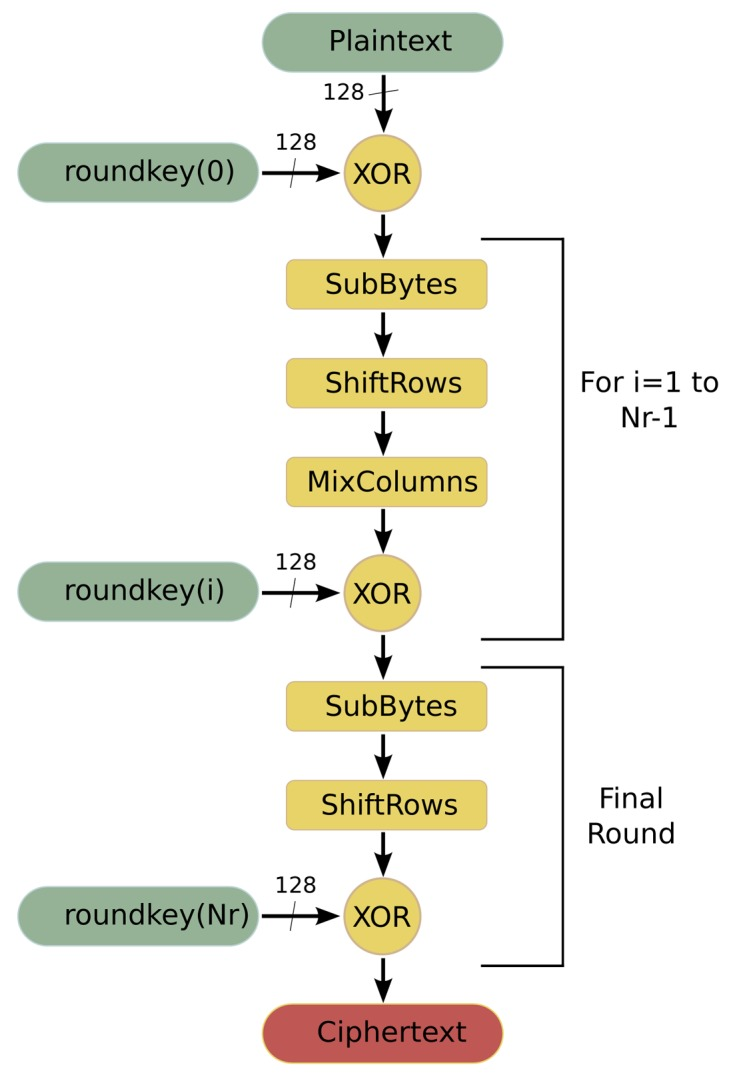
\includegraphics[scale=1.5]{AES_1}
	\end{center}
	
	\paragraph{Giải thuật Mã hóa}
	\begin{description}
	\item Khởi động vòng lặp
		\begin{enumerate}
			\item AddRoundKey — Mỗi cột của trạng thái đầu tiên lần lượt được kết hợp với một khóa con theo thứ tự từ đầu dãy khóa.
		\end{enumerate}
	\item Vòng lặp
		\begin{enumerate}
			\item SubBytes — đây là phép thế (phi tuyến) trong đó mỗi byte trong trạng thái sẽ được thế bằng một byte khác theo bảng tra (Rijndael S-box).
			\item ShiftRows — dịch chuyển, các hàng trong trạng thái được dịch vòng theo số bước khác nhau.
			\item MixColumns — quá trình trộn làm việc theo các cột trong khối theo một phép biến đổi tuyến tính.
			\item AddRoundKey
		\end{enumerate}
	\item Vòng lặp cuối
		\begin{enumerate}
			\item SubBytes
			\item ShiftRows
			\item AddRoundKey
		\end{enumerate}
	\end{description}
		\subsubsection{Hàm SubBytes()}
		Hàm SubBytes() thực hiện phép thay thế các byte của mảng trạng thái bằng cách sử dụng một bảng thế S-Box, bảng thế này là khả nghịch và được xây dựng bằng cách kết hợp 2 biến đối nhau:
		\begin{itemize}
		\item Nhân nghịch đảo trên trường hữu hạn GF ($2^8$), phần tử {00} được ánh xạ thành chính nó.
		\item Áp dụng biến đổi Affine sau (trên GF(2)): 
		\begin{center}
		$b^{'}_{i} = b_i \oplus b_{(i+4)mod 8} \oplus b_{(i+5)mod 8} \oplus b_{(i+6)mod 8} \oplus b_{(i+7)mod 8} \oplus c_i$
		\end{center}
		trong đó $0 \le i \le 8$ là bit thứ i của byte b tương ứng và $c_i$ là bit thứ i của byte c với giá trị \{63\} hay \{01100011\}	
		\end{itemize}
		Các phần tử biến đổi affine của S-box có thể được biểu diễn dưới dạng ma trận như sau :
		\begin{center}
		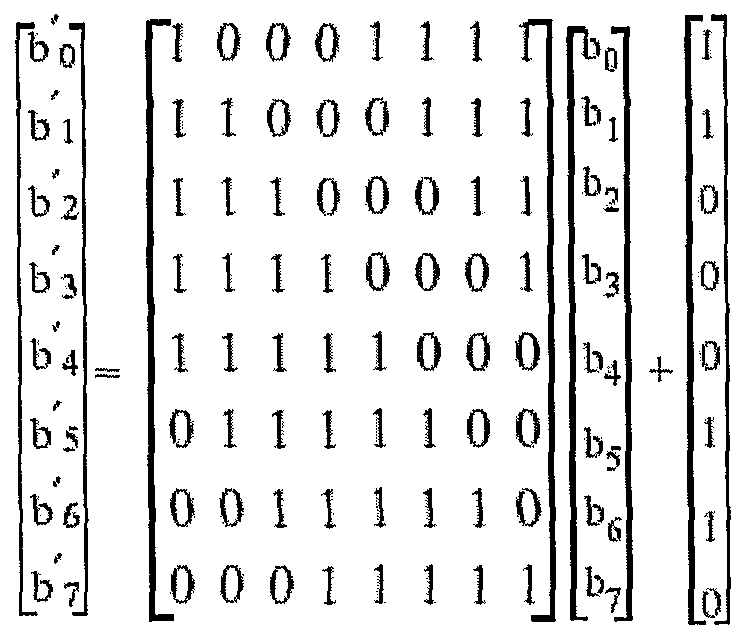
\includegraphics[scale=0.3]{AES_SBOX_1}
		\end{center}
		Hình sau minh họa kết quả của việc áp dụng hàm biến đổi SubBytes() đối với mảng trạng thái:
		\begin{center}
		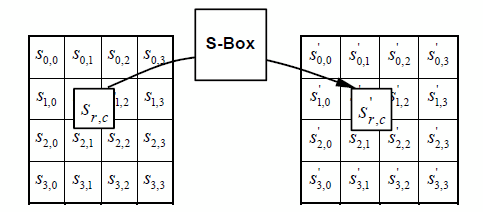
\includegraphics[scale=0.7]{AES_SBOX_2}
		\end{center}
		Bảng thế S-box được sử dụng trong hàm Subbytes() có thể được biểu diễn dưới dạng hexa như sau:
		\begin{center}
		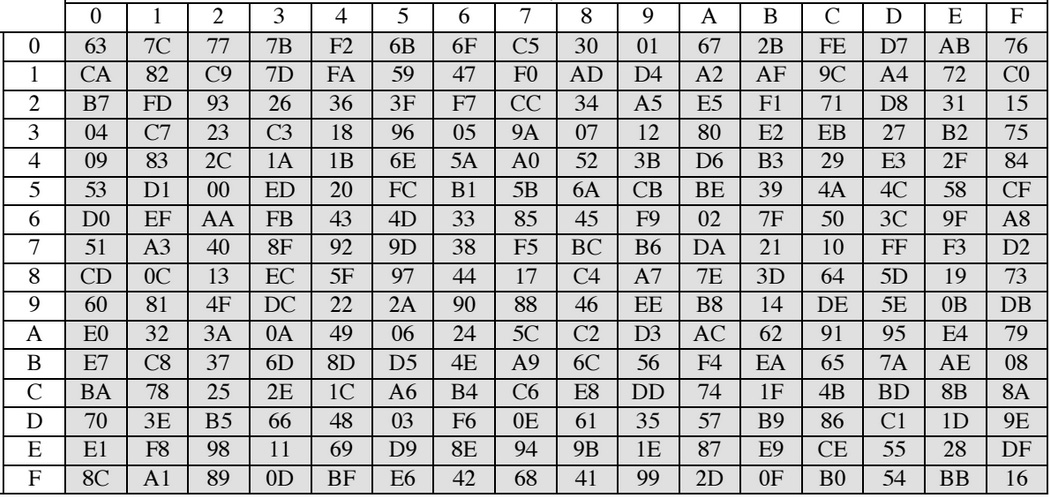
\includegraphics[scale=0.4]{AES3S-Box}
		\end{center}
		trong đó chẳng hạn nếu $S_{1,1}=\{53\}$ có nghĩa là giá trị thay thế sẽ được xác định bằng giao của hàng có chỉ số 5 với cột có chỉ số 3 trong bảng trên, điều này tương đương với việc $S^{'}_{1,1}=\{ed\}$
		\subsubsection{Hàm ShiftRows()}
		Là phép biến đổi các byte trên ba hàng cuối cùng của mảng trạng thái bằng cách dịch vòng thể hiện qua công thức:
		\begin{center}
		$S^{'}_{r,c}=S_{r,(c+shift(r,Nb)mod Nb)}$, với $ 0 < r \le 3$ và $0 \le c < Nb$
		\end{center}
		Số lần dịch vòng shift(r,Nb) phụ thuộc vào chỉ số vòng. Cụ thể shift(4,1)=1, shift(2,4)=1, shift(3,4)=3.
		\subsubsection{Hàm MixColumns()}
		MixColumns() là một phép biến đổi mã hóa được thực hiện bằng cách lấy tất cả các cột của Mảng trạng thái trộn với dữ liệu của chúng một cách độc lập nhau để tạo ra các cột mới.
		\begin{center}
		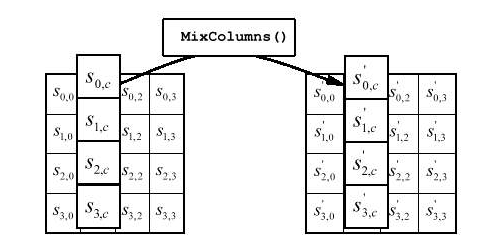
\includegraphics[scale=0.4]{AES4MIXCOLUME}
		\end{center}
		
		\subsubsection{Hàm AddRoundKey()}
		Trong biến đổi AddRoundKey(), một khóa vòng được cộng với state bằng 1 phép XOR theo từng bit đơn giản. Mỗi khóa vòng gồm có 4 từ (128bit) được lấy từ lược đố khóa. 4 từ đó được cộng vào state, sao cho:
		\begin{center}
		$[s^{'}_{0,c},s^{'}_{1,c},s^{'}_{2,c},s^{'}_{3,c}] = [s^{'}_{0,c},s^{'}_{1,c},s^{'}_{2,c},s^{'}_{3,c}] \oplus [W_{4*i+c}]$ với $0 \le c < 4$
		\end{center}
		Trong đó $w_{4*i+c}$ là các từ thứ c của khóa vòng thứ i
		\begin{center}
		$W_{i} = [w_{4*i},w_{4*i+1},w_{4*i+2},w_{4*i+3}]$
		\end{center}
		\begin{center}
		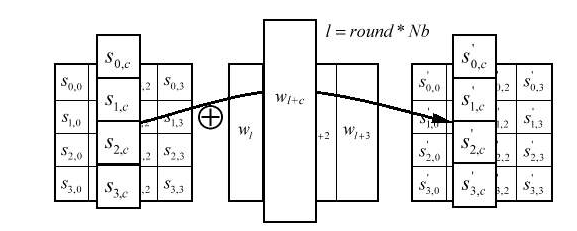
\includegraphics[scale=0.5]{AESADDROUNDKEY}
		\end{center}
	\paragraph{Giải thuật Giải mã}
		\subsubsection{Hàm InvShiftRows()}
		Hàm này là hàm ngược cùa hàm ShiftRows(). Các byte của ba hàng cuối của mảng trạng thái sẽ được dịch vòng với các vị trí dịch khác nhau. Hàng đầu tiên không bị dịch, ba hàng cuối bị dịch đi Nb-Shift(r,Nb) byte.\\
		Cụ thể hàm này tiến hành xử lý như sau:
		\begin{center}
		$S^{'}_{r,(c+shift(r,Nb))mod Nb} = S_{r,c}$ với $ 0 < r < 4, 0 \le c < Nb$
		\end{center}
		\begin{center}
		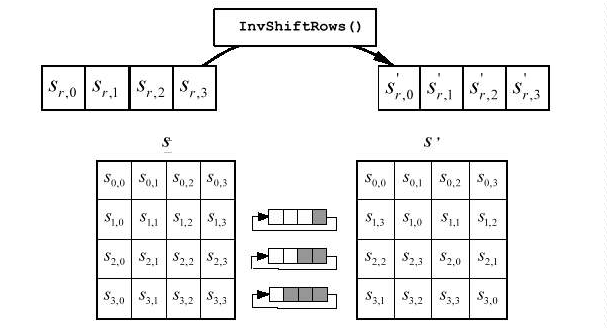
\includegraphics[scale=0.7]{AESSHIFT}
		\end{center}

		\subsubsection{Hàm InvSubytes()}
		Hàm này là hàm ngược của hàm SubBytes(), hàm sử dụng nghịch đảo của biến đổi Affine bằng cách thực hiện nhân nghịch đảo trên $GF(2^2)$\\
		Bảng thế được sử dụng trong hàm:
		\begin{center}
		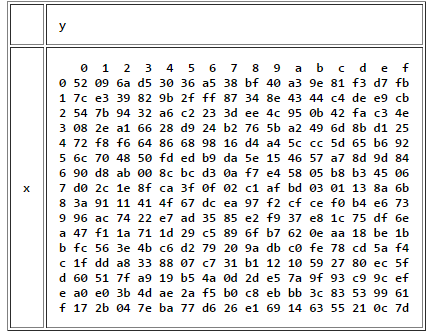
\includegraphics[scale=0.6]{AESInvSubByte}
		\end{center}
		\subsubsection{Hàm InvMixColumns()}
		Hàm này là hàm ngược của hàm MixColumns(). Hàm làm việc trên các cột của mảng trạng thái, coi mỗi cột như là một đa thức 4 hạng tử. Các cột được xem là các đa thức trên GF($2^8$) và được nhân theo modulo $x^4 +1$ với một đa thức cố định là $a^{-1}(x)$
		\begin{center}
		$a^{-1} = \{0b\}x^3 +\{0d\}x^2 + \{09\}x + \{0e\}$
		\end{center}
		Và có thể mô tả bằng phép nhân ma trận như sau:
		\begin{center}
		$S^{'}(x) = a^{-1}x \otimes S(x)$
		\end{center}
		\begin{center}
		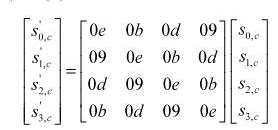
\includegraphics[scale=0.6]{AESMixColume}
		\end{center}
		Trong đó $0 \le c < Nb$.\\
		Kết quả là bốn byte trong mỗi cột sẽ được thay thế theo công thức sau :
		\begin{center}
		$S^{'}_{0,c}=(\{0e\} \bullet S_{0,c})\oplus (\{0b\} \bullet S_{1,c})\oplus (\{0d\} \bullet S_{2,c})\oplus (\{09\} \bullet S_{3,c})\oplus$ \\
		$S^{'}_{1,c}=(\{09\} \bullet S_{0,c})\oplus (\{0e\} \bullet S_{1,c})\oplus (\{0b\} \bullet S_{2,c})\oplus (\{0d\} \bullet S_{3,c})\oplus$ \\
		$S^{'}_{2,c}=(\{0d\} \bullet S_{0,c})\oplus (\{09\} \bullet S_{1,c})\oplus (\{0e\} \bullet S_{2,c})\oplus (\{0b\} \bullet S_{3,c})\oplus$ \\
		$S^{'}_{3,c}=(\{0b\} \bullet S_{0,c})\oplus (\{0d\} \bullet S_{1,c})\oplus (\{09\} \bullet S_{2,c})\oplus (\{0e\} \bullet S_{3,c})\oplus$ 
		\end{center}
		\subsubsection{Hàm nghịch đảo của hàm AddRoundKey()}
		Thật thú vị là hàm này tự bản thân nó là nghịch đảo của chính nó là do hàm chỉ có phép toán XOR bit.
		\newpage
\subsection {Thuật toán mã hóa DES.}
DES (viết tắt của Data Encryption Standard, hay Tiêu chuẩn Mã hóa Dữ liệu) là một phương pháp mật mã hóa được FIPS (Tiêu chuẩn Xử lý Thông tin Liên bang Hoa Kỳ) chọn làm chuẩn chính thức vào năm 1976. Sau đó chuẩn này được sử dụng rộng rãi trên phạm vi thế giới. Ngay từ đầu, thuật toán của nó đã gây ra rất nhiều tranh cãi, do nó bao gồm các thành phần thiết kế mật, độ dài khóa tương đối ngắn, và các nghi ngờ về cửa sau để Cơ quan An ninh quốc gia Hoa Kỳ (NSA) có thể bẻ khóa. Do đó, DES đã được giới nghiên cứu xem xét rất kỹ lưỡng, việc này đã thúc đẩy hiểu biết hiện đại về mật mã khối (block cipher) và các phương pháp thám mã tương ứng.\\[1cm]
Mô tả giải thuật\\[0.5cm]
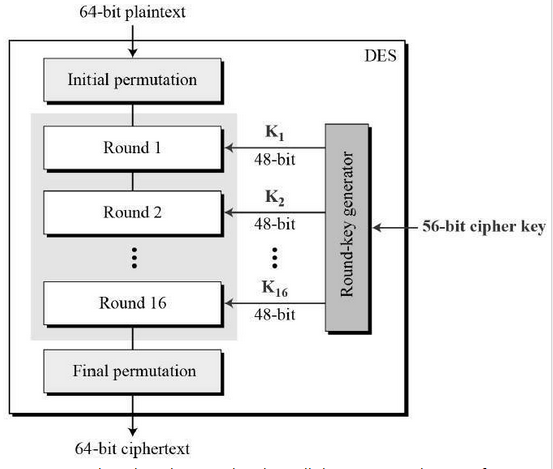
\includegraphics[scale=0.8]{DES}\\
DES là thuật toán mã hóa khối: nó xử lý từng khối thông tin của bản rõ có độ dài xác định và biến đổi theo những quá trình phức tạp để trở thành khối thông tin của bản mã có độ dài không thay đổi. Trong trường hợp của DES, độ dài mỗi khối là 64 bit. DES cũng sử dụng khóa để cá biệt hóa quá trình chuyển đổi. Nhờ vậy, chỉ khi biết khóa mới có thể giải mã được văn bản mã. Khóa dùng trong DES có độ dài toàn bộ là 64 bit. Tuy nhiên chỉ có 56 bit thực sự được sử dụng; 8 bit còn lại chỉ dùng cho việc kiểm tra. Vì thế, độ dài thực tế của khóa chỉ là 56 bit.
Giống như các thuật toán mã hóa khối khác, khi áp dụng cho các văn bản dài hơn 64 bit, DES phải được dùng theo một phương pháp nào đó. Trong tài liệu FIPS-81 đã chỉ ra một số phương pháp, trong đó có một phương pháp dùng cho quá trình nhận thực. Một số thông tin thêm về những cách sử dụng DES được miêu tả trong tài liệu FIPS-74 .

\begin{itemize}
    \item \textbf{Tổng thể:}\\[0.1cm]
   
 Cấu trúc tổng thể của thuật toán được thể hiện ở Hình 1: có 16 chu trình giống nhau trong quá trình xử lý. Ngoài ra còn có hai lần hoán vị đầu và cuối (Initial and final permutation - IP & EP). Hai quá trình này có tính chất đối nhau (Trong quá trình mã hóa thì IP trước EP, khi giải mã thì ngược lại). IP và EP không có vai trò xét về mật mã học và việc sử dụng chúng chỉ có ý nghĩa đáp ứng cho quá trình đưa thông tin vào và lấy thông tin ra từ các khối phần cứng có từ thập niên 1970. Trước khi đi vào 16 chu trình chính, khối thông tin 64 bit được tách làm hai phần 32 bit và mỗi phần sẽ được xử lý tuần tự (quá trình này còn được gọi là mạng Feistel).\\[0.1cm]
Cấu trúc của thuật toán (mạng Feistel) đảm bảo rằng quá trình mã hóa và giải mã diễn ra tương tự. Điểm khác nhau chỉ ở chỗ các khóa con được sử dụng theo trình tự ngược nhau. Điều này giúp cho việc thực hiện thuật toán trở nên đơn giản, đặc biệt là khi thực hiện bằng phần cứng.\\[0.1cm]
 Ký hiệu sau: thể hiện phép toán XOR. Hàm F làm biến đổi một nửa của khối đang xử lý với một khóa con. Đầu ra sau hàm F được kết hợp với nửa còn lại của khối và hai phần được tráo đổi để xử lý trong chu trình kế tiếp. Sau chu trình cuối cùng thì 2 nửa không bị tráo đổi; đây là đặc điểm của cấu trúc Feistel khiến cho quá trình mã hóa và giải mã trở nên giống nhau.\\
    
    \item \textbf{Hàm Feistel (F):}\\[0.1cm]
    Hàm F, hoạt động trên khối 32 bit và bao gồm bốn giai đoạn:\\
    \begin{itemize}
        \item \emph{Mở rộng}: 32 bit đầu vào được mở rộng thành 48 bit sử dụng thuật toán hoán vị mở rộng (expansion permutation) với việc nhân đôi một số bit. Giai đoạn này được ký hiệu là E trong sơ đồ. \item \emph{Trộn khóa}: 48 bit thu được sau quá trình mở rộng được XOR với khóa con. Mười sáu khóa con 48 bit được tạo ra từ khóa chính 56 bit theo một chu trình tạo khóa con (key schedule) miêu tả ở phần sau.
        \item \emph{Thay thế}: 48 bit sau khi trộn được chia làm 8 khối con 6 bit và được xử lý qua hộp thay thế S-box. Đầu ra của mỗi khối 6 bit là một khối 4 bit theo một chuyển đổi phi tuyến được thực hiện bẳng một bảng tra. Khối S-box đảm bảo phần quan trọng cho độ an toàn của DES. Nếu không có S-box thì quá trình sẽ là tuyến tính và việc thám mã sẽ rất đơn giản.
        \item \emph{Hoán vị}: Cuối cùng, 32 bit thu được sau S-box sẽ được sắp xếp lại theo một thứ tự cho trước (còn gọi là P-box).
        
    \end{itemize}
   
Quá trình luân phiên sử dụng S-box và sự hoán vị các bít cũng như quá trình mở rộng đã thực hiện được tính chất gọi là sự xáo trộn và khuyếch tán (confusion and diffusion). Đây là yêu cầu cần có của một thuật toán mã hoá được Claude Shannon phát hiện trong những năm 1940.
    
    \item \textbf{Quá trình tạo khóa con :} \\
    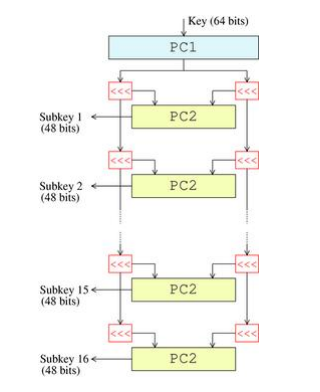
\includegraphics{DES_KEY}\\
    Đầu tiên, từ 64 bit ban đầu của khóa, 56 bit được chọn (Permuted Choice 1, hay PC-1); 8 bit còn lại bị loại bỏ. 56 bit thu được được chia làm hai phầnbằng nhau, mỗi phần được xử lý độc lập. Sau mỗi chu trình, mỗi phần được dịch đi 1 hoặc 2 bit (tùy thuộc từng chu trình). Các khóa con 48 bit được tạo thành bởi thuật toán lựa chọn 2 (Permuted Choice 2, hay PC- 2) gồm 24 bit từ mỗi phần. Quá trình dịch bit (được ký hiệu là "<<<" trong sơ đồ) khiến cho các khóa con sử dụng các bit khác nhau của khóa chính; mỗi bit được sử dụng trung bình ở 14 trong tổng số 16 khóa con.
    
    Quá trình tạo khóa con khi thực hiện giải mã cũng diễn ra tương tự nhưng các khóa con được tạo theo thứ tự ngược lại. Ngoài ra sau mỗi chu trình, khóa sẽ được dịch phải thay vì dịch trái như khi mã hóa
\end{itemize}

\subsection{Thuật toán mã hóa RSA}
Trong mật mã học , RSA là một thuật toán mã hóa khóa công khai .Đây là thuật toán đầu tiên phù hợp với việc tạo ra chữ ký điện tử đồng thời với việc mã hóa .Nó đánh dấu một sự tiến bộ vượt bậc của lĩnh vực mật mã học trong việc sử dụng khóa công cộng .RSA đang được sử dụng phổ biến trong thương mại điện tử và được cho là đảm bảo an toàn với diiều kiện độ dài khóa đủ lớn .
\begin{itemize}
    \item \textbf{Tổng thể:}\\[0.1cm]


Thuật toán được Ron Rivest , Adi Shamir và Len Adleman mô tả lần đầu tiên vào năm 1977 tại học viện Công nghệ  Massachusetts ( MIT) . Tên của thuật toán lấy từ 3 chữ cái đầu tiên của 3 tác giả .\\
	
	
Trước đó , vào năm 1973 ,Clifford Cocks , một nhà toán học người Anh làm việc tại GCHQ đã mô tả một thuật toán tương tự . Với khả năng tính toán tại thời điểm đó thì thuật toán này không khả thi và chưa bao giờ được thực nghiệm .Tuy nhiên , phát minh này chỉ được công bố vào năm 1997 vì được xếp vào loại tuyệt mật \\


Thuật toán RSA được MIT đăng ký bằng sáng chế tại Hoa Kỳ vào năm 1983.Tuy nhiên , do thuật toán đã được công bố trước khi có đăng ký bảo hộ nên sự bảo hộ hầu như không có giá trị bên ngoài Hoa Kỳ .Ngoài ra , nếu như công trình của Clifford Cocks đã công bố trước đó thì bằng sáng chế RSA đã không thể được đăng ký .
\\
\end{itemize}
\begin{itemize}
    \item \textbf{Tạo Khóa:}\\[0.1cm]
	Gọi p và q là hai số nguyên tố lớn ngẫu nhiên phân biệt.\\

	Modun n là tích của hai số nguyên tố này:

	\begin{center}
		$n = pq$
	\end{center}

	Hàm phi Euler (Euler's totient function) của n cho bởi:
	\begin{center}
		$\phi{(n)} = (p-1)(q-1)$
	\end{center}

	Chọn một số 1<e<$\phi{(n)}$ sao cho:
	\begin{center}
		$gcd(e, \phi{(n)}) = 1$
	\end{center}

	và tính d với công thức:

	\begin{center}
		$d = e^{-1} mod \: \phi{(n)}$
	\end{center}

	Việc mã hóa được thực hiện bằng cách tính:

	\begin{center}
		$C = M^{e} \: (mod \: n)$
	\end{center}

	với M là plaintext, C là ciphertext tương ứng của M.\\
	Từ C, M được tính bằng công thức:

	\begin{center}
		$M = C^{d} \: (mod \: n)$\\
	\end{center}
	\end{itemize}
	\subsection{Hàm băm MD-5}
	MD5 chuyển một đoạn thông tin chiều dài thay đổi thành một kết quả chiều dài không đổi 128 bit. Mẩu tin đầu vào được chia thành từng đoạn 512 bit; mẩu tin sau đó được độn sao cho chiều dài của nó chia chẵn cho 512. Công việc độn vào như sau: đầu tiên một bit đơn, 1, được gắn vào cuối mẩu tin. Tiếp theo là một dãy các số zero sao cho chiều dài của mẩu tin lên tới 64 bit ít hơn so với bội số của 512. Những bit còn lại được lấp đầy bằng một số nguyên 64-bit đại diện cho chiều dài của mẩu tin gốc.

		
		
\section{Nội dung công việc đã làm.}
 
 %%%%%%%%%%%%%%%%%%%%%%%%%%%%%%%%%%%%%%%%%%%%%%%%%%%%%%%%%%%%%%%%%%%%%%%%%%%%%%%%%%%%%%%%%%%%%%%%%%%%%%%

\subsection{Thuật toán mã hóa AES}
	Cơ bản bao gồm các hàm mã hóa-giải mã và hàm sinh key
	
	\begin{enumerate}
	\item \emph{private byte[]} Encrypt(\emph{byte[]} clearData, \emph{byte[]} Key, \emph{byte[]} IV): mã hóa một mãng byte dữ liệu vào bằng key và IV.

    \item \emph{private void} \excludecomment {AESAlgorithm(String inputFile, String OutputFile, String keys, bool isEncrypt, String mode) \\Đây là hàm dùng để mã hóa và giải mã một file bất kỳ.Với các thông số truyền vào là đường dẫn file input, chuỗi khóa (key) ,mode có thể là các chế độ như : ECB,CBC,CFB và thông số isEncrypt=true nếu đây là quá trình mã hóa và ngược lại.} 
    
  
\item Và một số hàm hổ trợ khác.

\item $Và private void btnGenerateKey_Click ( object sender, EventArgs e )$

	\end{enumerate}
 %%%%%%%%%%%%%%%%%%%%%%%%%%%%%%%%%%%%%%%%%%%%%%%%%%%%%%%%%%%%%%%%%%%%%%%%%%%%%%%%%%%%%%%%%%%%%%%%%%%%%%%
\subsection{Thuật toán mã hóa RSA}
Gồm 2 hàm quan trọng nhất là encrypt và decrypt:\\
Đầu tiên chúng ta dùng hàm ConvertFileByte() để chuyển file cần mã hóa thành dạng byte():\\
      \begin{center}
	\emph{public static} byte[] ConvertFileToByte(\emph{string} \_FileName)\{…\}
	\end{center}
Dùng công cụ để chuyển mảng byte đó thành dạng hexadecimal string, sau đó dùng hàm encrypt() để mã hóa thuật toán RSA.\\
       \begin{center}
	\emph{public string} encrypt(\emph{string} FileToEncrypt)
	\end{center}
Ở đây, hàm BigMod() có vai trò mã hóa theo công thức:  
File mã hóa xong có định dạng txt chứa thông tin của file cần mã hóa dưới dạng các chuổi hexademical string.\\ \\
	Hàm decrypt có nhiệm vụ giải mã theo thuật toán RSA, trong đó hàm BigMod() ở đây có nhiệm vụ giải mã theo công thức: $ m = c^d \hspace{0.2cm} mod \hspace{0.2cm} N$
	\begin{center}
	\emph{public string} decrypt(\emph{string} FileToEncrypt)
	\end{center}
	Sau đó, ta dùng hàm ConvertByteToFile() để chuyển mảng Byte thành File như ban đầu.\\
	
	Ngoài ra, ta còn sử dụng hàm hỗ trợ auto\_prime\_number() để sinh khóa tự động, giảm thời gian cho việc thao tác.
 %%%%%%%%%%%%%%%%%%%%%%%%%%%%%%%%%%%%%%%%%%%%%%%%%%%%%%%%%%%%%%%%%%%%%%%%%%%%%%%%%%%%%%%%%%%%%%%%%%%%%%%
\subsection{Thuật toán mã hóa DES} 
Chứa cả 2 phần mã hóa và giải mã, dữ liệu đầu vào là file input, key với độ dài 64bit,
mode ở đây có thể là ECB,CBC,CFB. isEncrypt có kiểu bool nếu isEncrypt = True là giải mã, ngược lại thì mã hóa.\\

void DESAlgorithm(string sInputFilename, string sOutputFilename, string sKey, string mode, bool isEncrypt)


 %%%%%%%%%%%%%%%%%%%%%%%%%%%%%%%%%%%%%%%%%%%%%%%%%%%%%%%%%%%%%%%%%%%%%%%%%%%%%%%%%%%%%%%%%%%%%%%%%%%%%%%
\subsection{Hàm băm MD5}
Nhóm đã sử dụng thư viện mã hóa trong C\# là :\hspace{0.2cm}\emph{System.Security.Cryptography}  \\
	Hàm chính để mã hóa dữ liệu :
	\begin{enumerate}
	\item \emph{private string} GetMD5HashData(\emph{string} data): nhận vào chuỗi dữ liệu và trả về chuỗi string có chiều dài nhất định.
	\item \emph{private string} openfile(): hàm phân tích file thành các blocksize trả về giá chuổi string là đầu vào của hàm GetMD5HashData
	\end{enumerate}
	\newpage
 %%%%%%%%%%%%%%%%%%%%%%%%%%%%%%%%%%%%%%%%%%%%%%%%%%%%%%%%%%%%%%%%%%%%%%%%%%%%%%%%%%%%%%%%%%%%%%%%%%%%%%% 

 
\section{Demo chương trình}
\textbf {Giao diện chính của chương trình}.\\

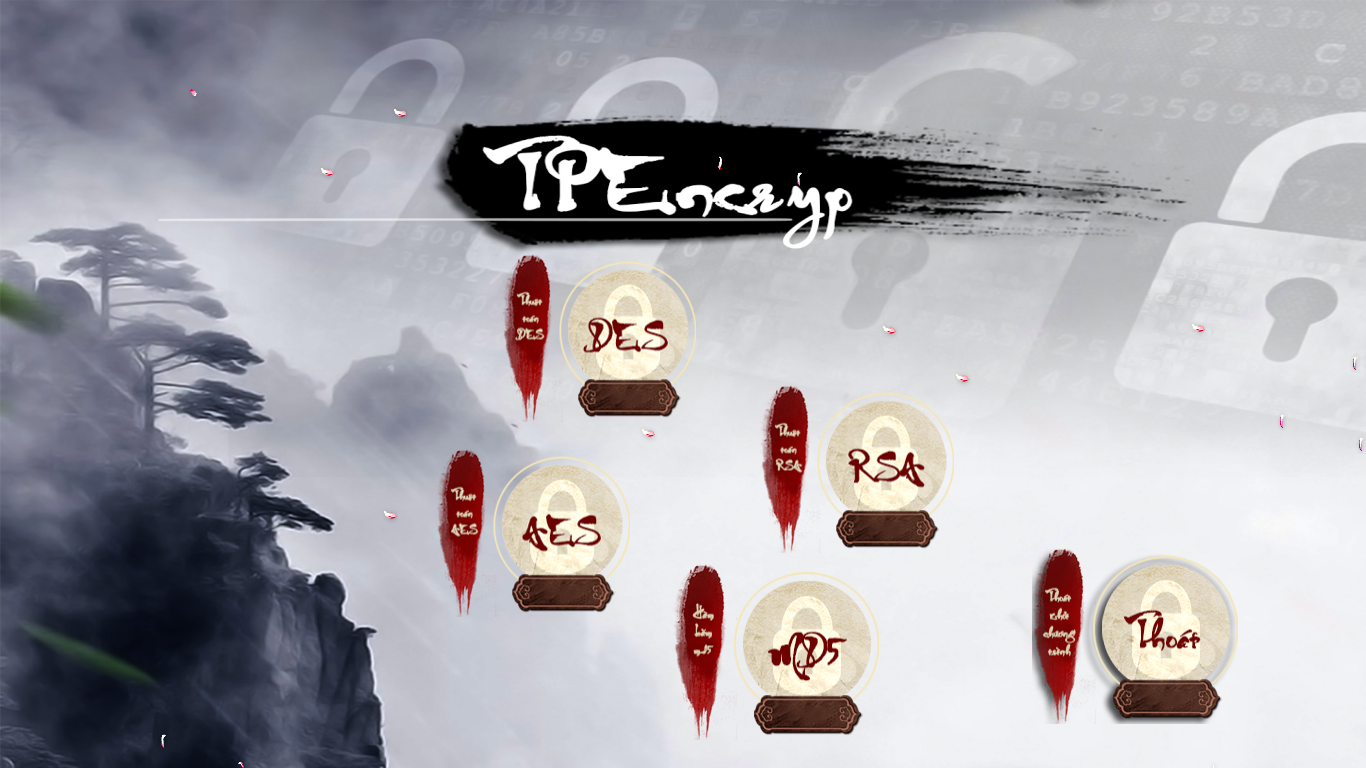
\includegraphics[scale = 0.4]{backroud}

 	\subsection{Giải thuật mã hóa DES  (DES)}
 	Giao diện chính gồm 2 phần Encrypt và Decrypt.\\
 
		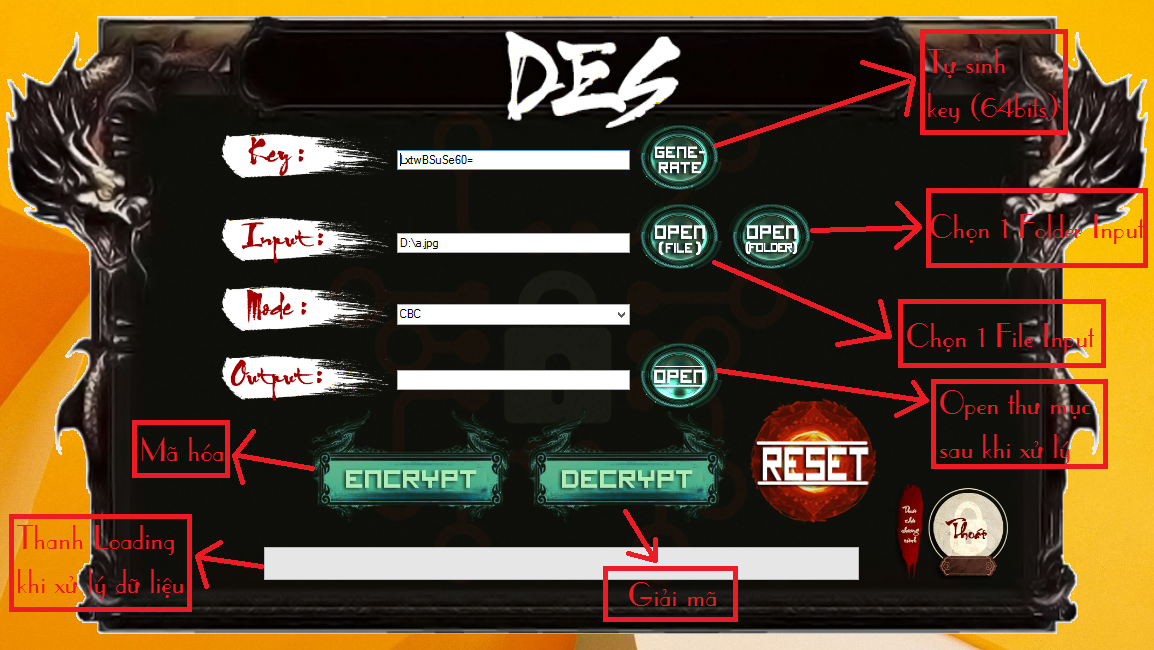
\includegraphics[scale=0.4]{DES_Chucnang}

 		\subsubsection{Phần mã hóa}
 		
 	    Phần Input File : có thể mã hóa hầu hết tất cả các file như: hình ảnh, âm thanh, video, pdf, các file dạng văn bản… Còn có thể mã hóa tập tin nén dạng zip,thư mục,rar.\\
 	
 	
		Phần Input Key : có thể nhập key bất kỳ có chiều dài 64bit(8byte) hoặc chọn Generate để random một key bất kì.\\
		
		
		Phần Output File: mật định chọn nơi lưu file ciphertext là nơi chọn file plaintext để mã hóa, file ciphertext có đuôi .tpEn\\
	    
	
		Ấn Encrypt để tiến hành mã hóa.\\
		
		Giao diện sau khi mã hóa thành công.\\
		
		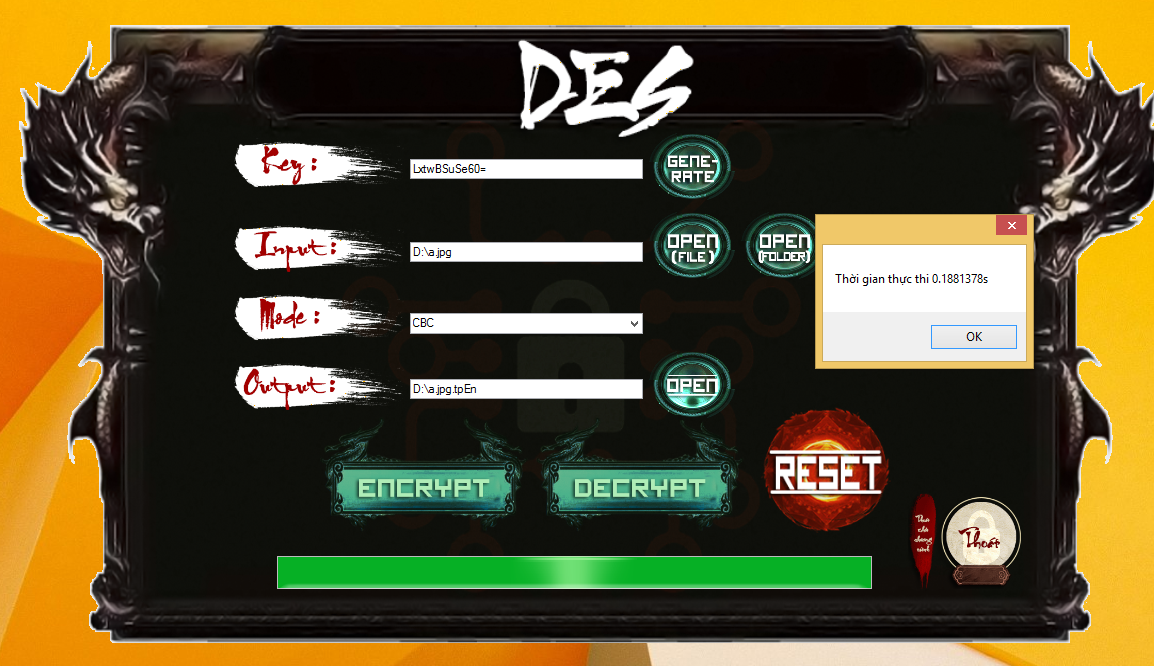
\includegraphics[scale=0.4]{DES_END}
 		\subsubsection{Phần giải mã}
 		
 		Phần Input File: chọn file có đuôi .tpEn để giải mã.\\
 	
 	
		Phần Input Key: nhập key ở phần mã hóa.\\
	
	
		Phần Output File: xuất ra file plaintext ban đầu.\\
	
	
		Ấn Decrypt để tiến hành giải mã.\\
		
		
		
	\subsection{Thuật toán mã hóa RSA}
		{Giao diện chính của giải thuật RSA} .\\
		
		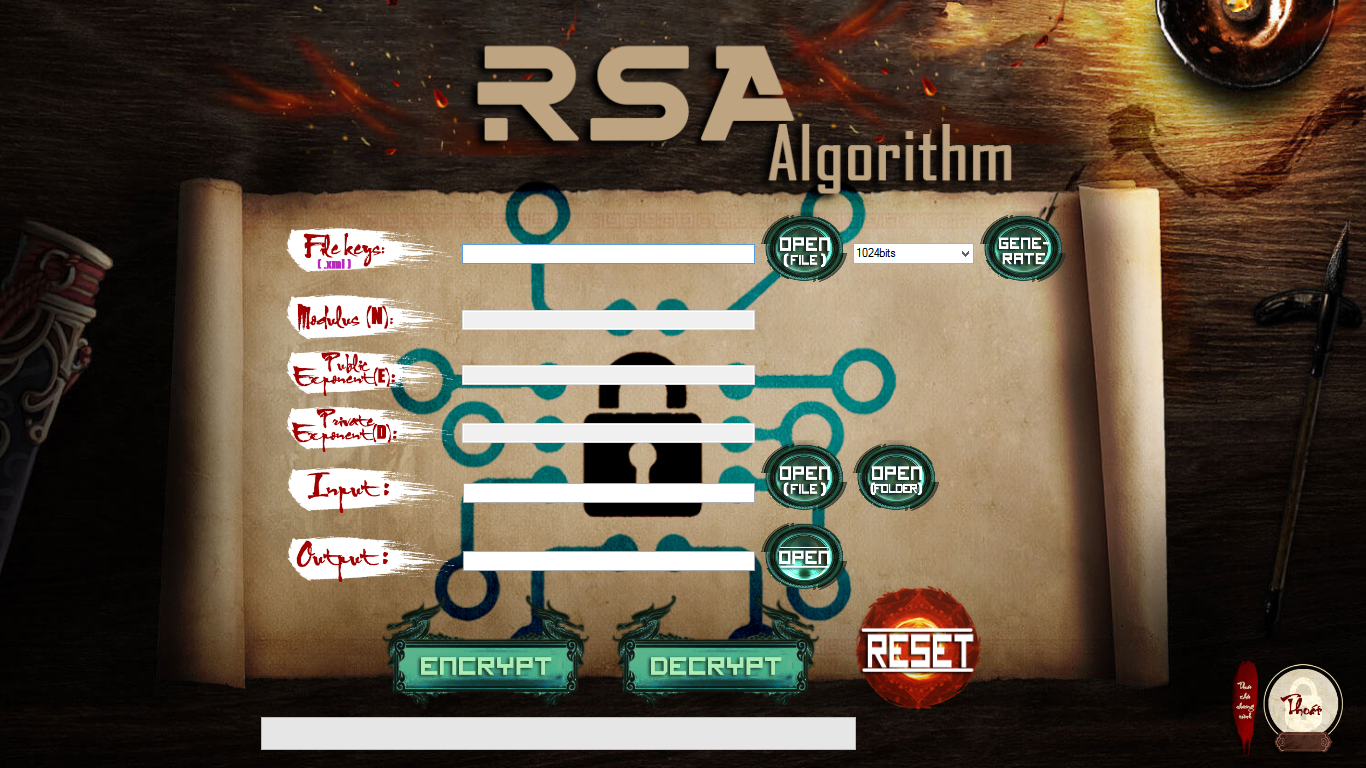
\includegraphics[scale=0.4]{RSA_GiaoDien}
		
		\subsubsection{Phần mã hóa}
		Mô tả tính năng : \\
		
		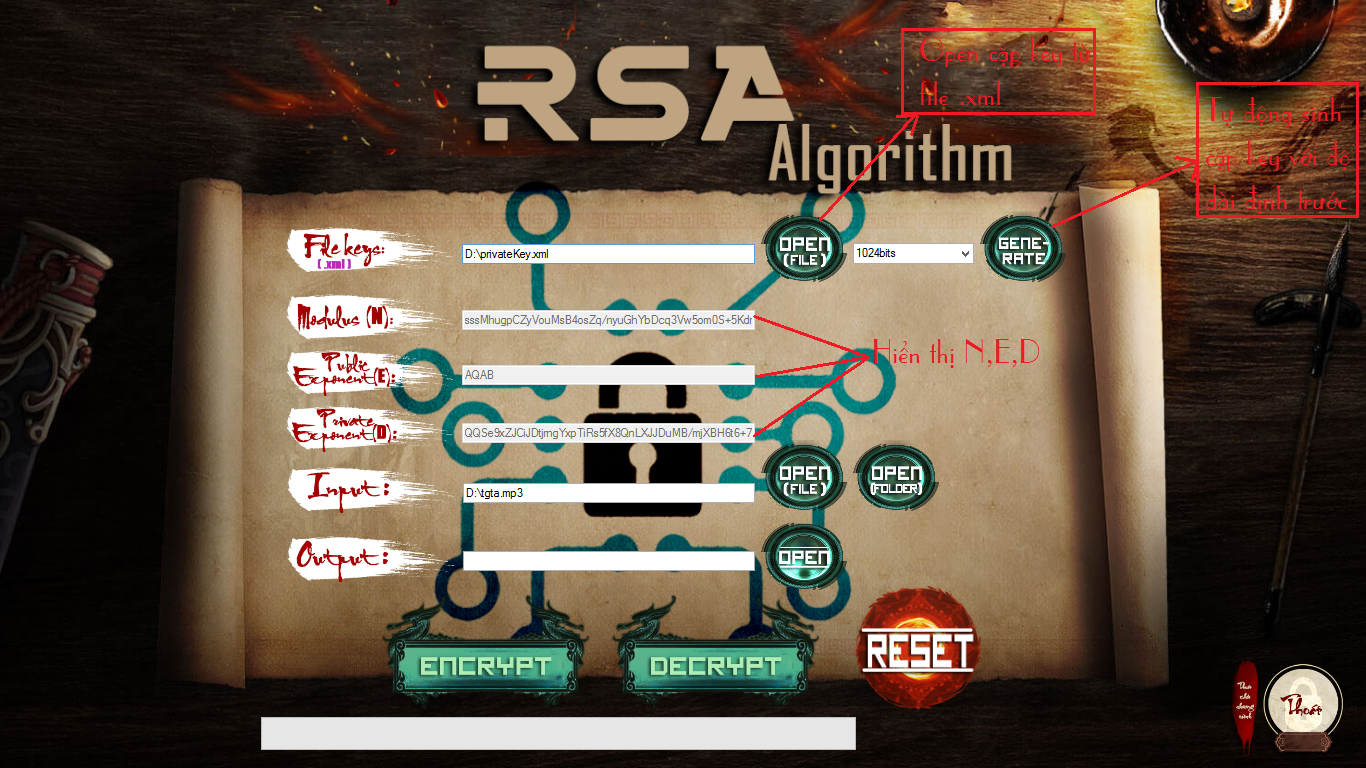
\includegraphics[scale = 0.4]{RSA_MOTA}
	    
	    Ngay File key nhấn vào open để mở tập file key từ file .xml hoặc nhấn generate để sinh ra file key định dạng .xml. Sau đó chọn file input để mã hóa.\\
	    
	    Giao diện sau khi mã hóa.\\
	    
	    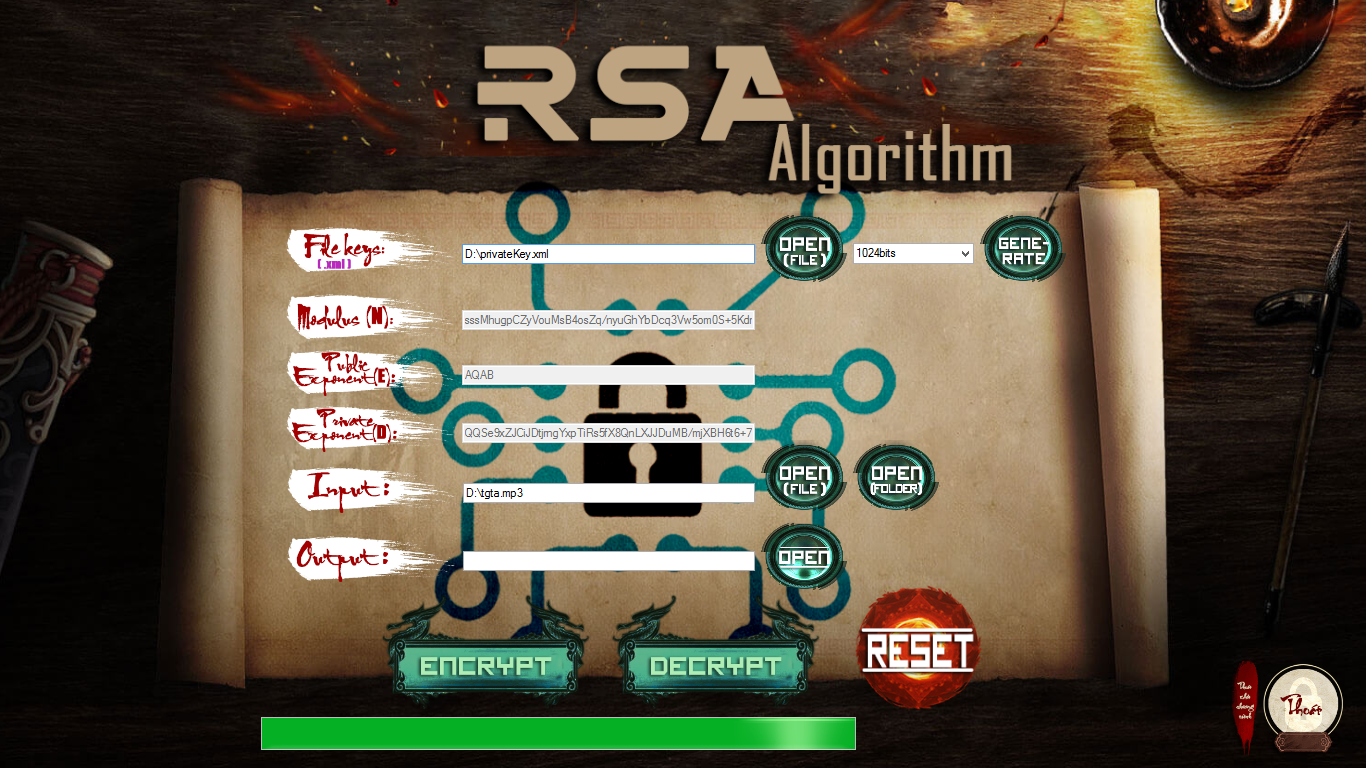
\includegraphics[scale = 0.4]{RSA_END}

		\subsubsection{Phần giải mã}
		Tương tự như phần mã hóa. Chỉ khác ngay phần input là định dạng file .tpEn \\
		
		 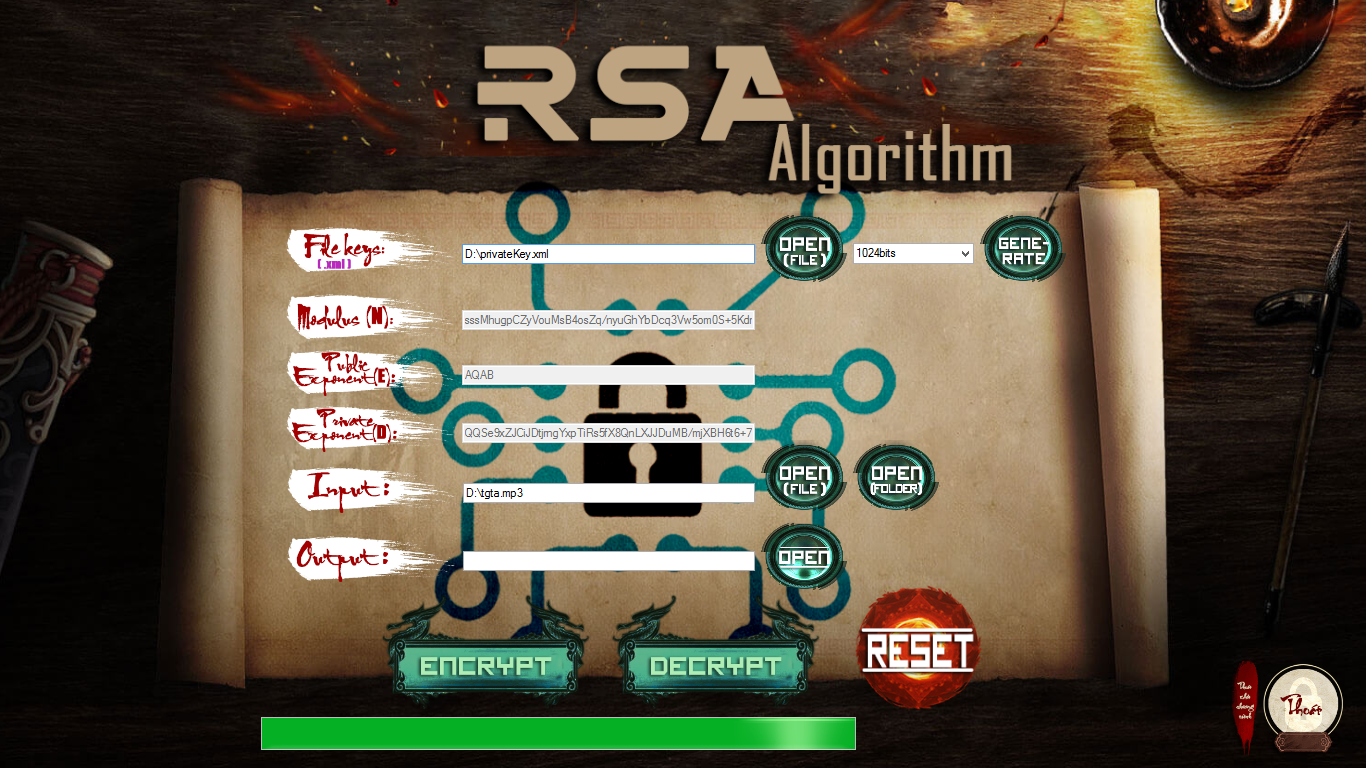
\includegraphics[scale = 0.4]{RSA_END}
		
	\subsection{Hàm băm MD-5}
	Giao diện chính gồm 2 phần File và Text:
	\begin{center}
		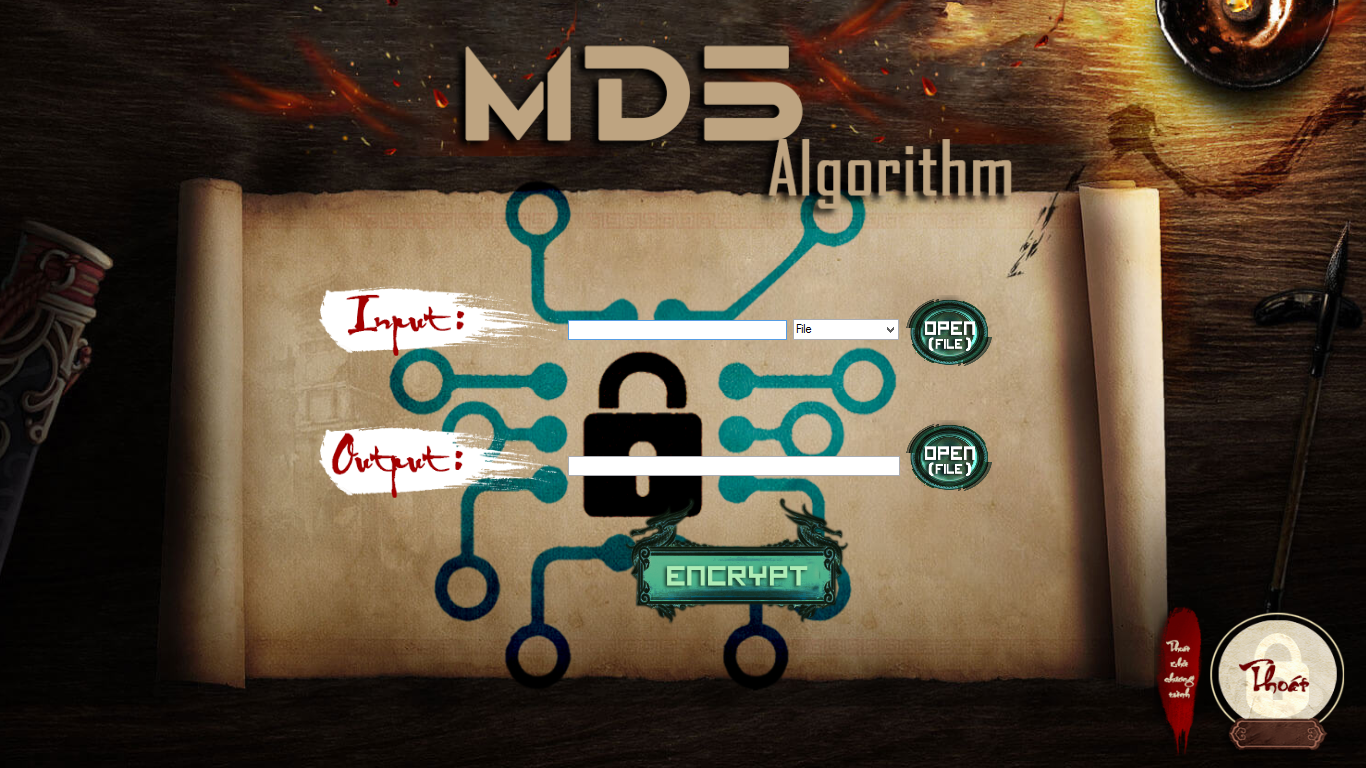
\includegraphics[scale=0.4]{MD5GIAODIEN}
	\end{center}
	
 	   \subsubsection{Phần file}
 		Phần Input Path: có thể mã hóa hầu hết tất cả các file như: hình ảnh, âm thanh, video, pdf, các file dạng văn bản… Còn có thể mã hóa tập tin nén dạng zip,rar,thư mục…
 			\begin{center}
				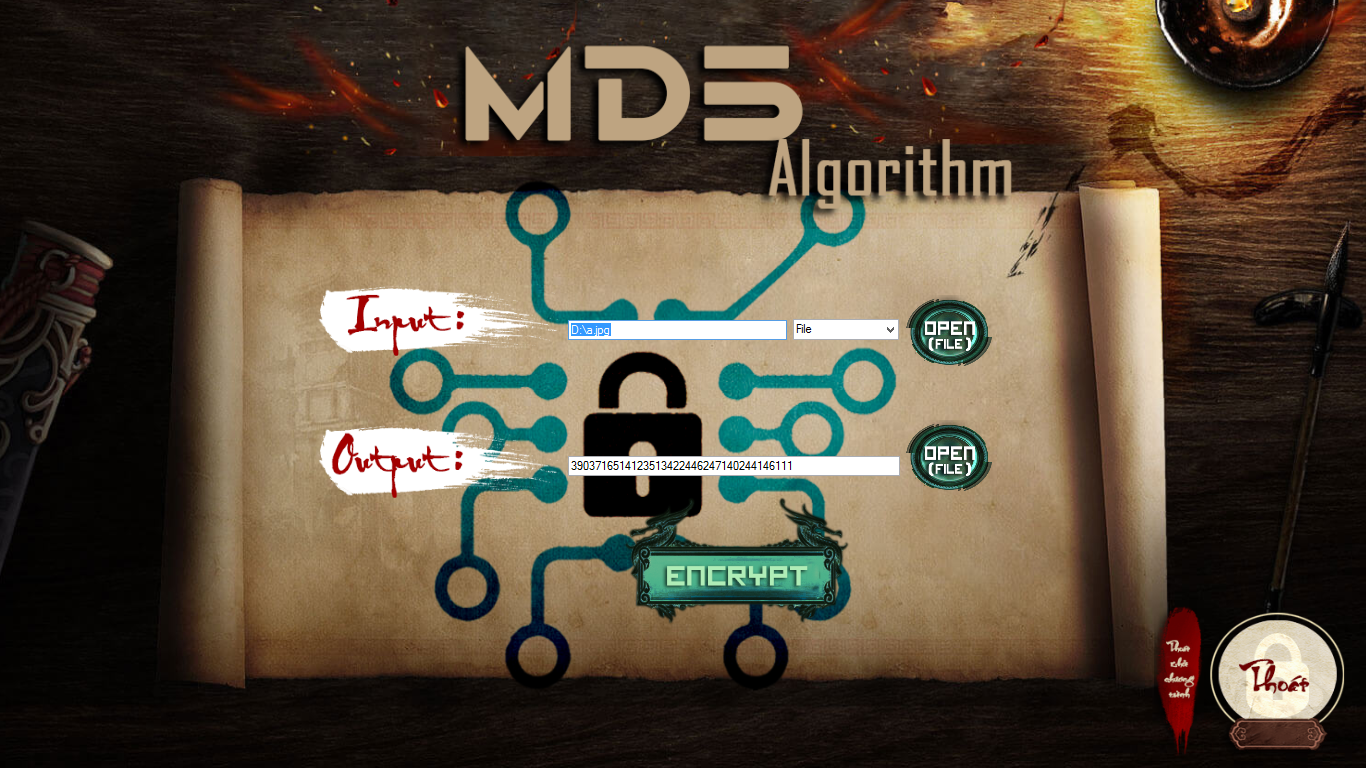
\includegraphics[scale=0.4]{MD5MAHOAFILE}
			\end{center}
		Phần Output Path: giá trị sao khi băm.\\
		
		Ấn Encypt để bắt đầu mã hóa\\
		
		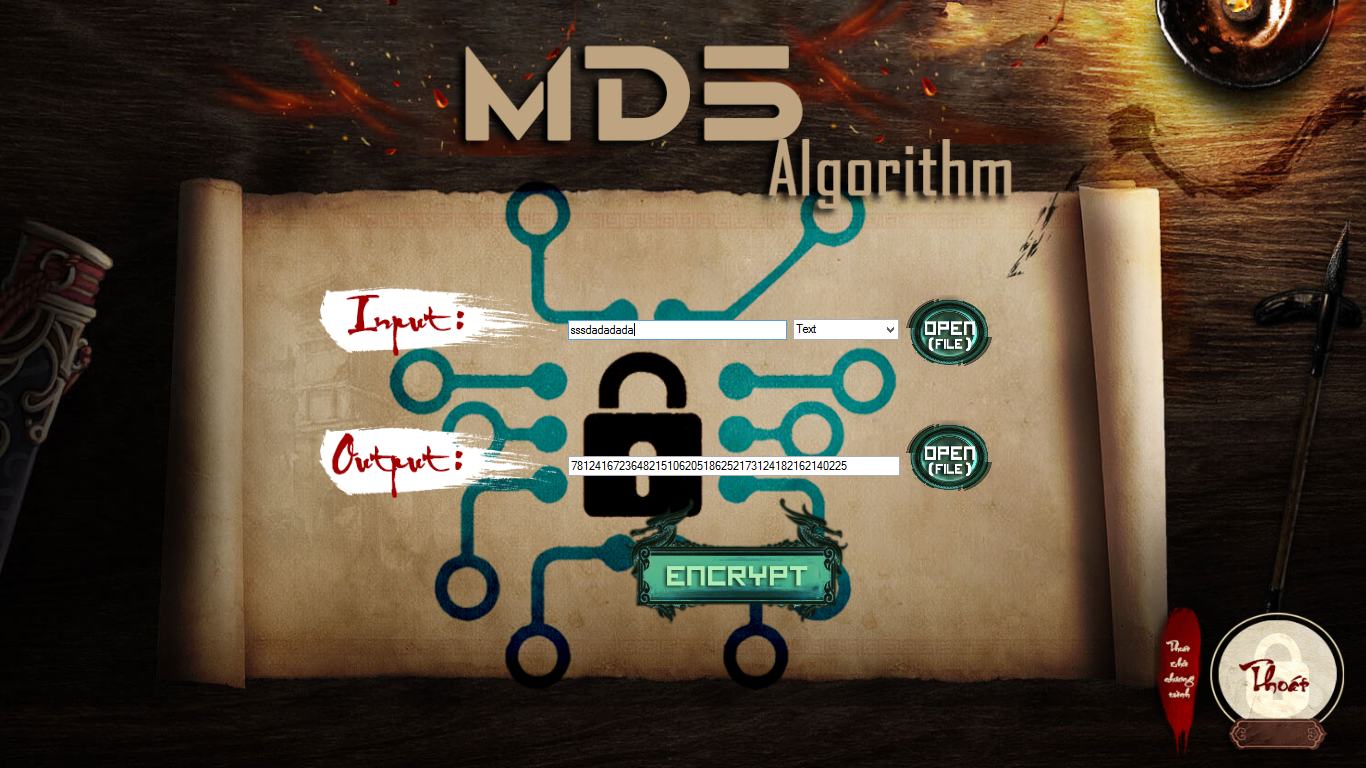
\includegraphics[scale=0.4]{MD5TEXT}
 		\subsubsection{Phần text}
 		Phần Input Path: Nhập vào đoạn text, hay một key cần mã hóa
 		
		Phần Output Path: giá trị sao khi mã hóa.\\
			
		Ấn Encrypt để bắt đầu mã hóa.\\
		
	\subsection{Giải thuật mã hóa AES}
	Giao diện chính gồm 2 phần Encrypt và Decrypt:\\
	
		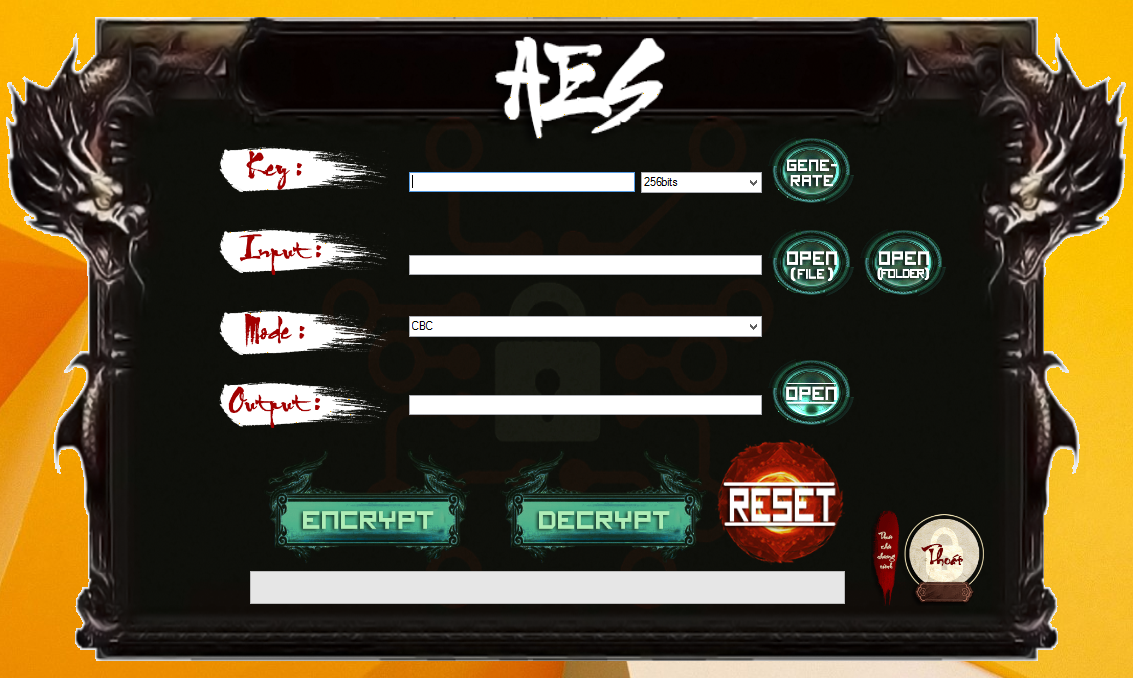
\includegraphics[scale=0.4]{AES_BACKROUND}

 		\subsubsection{Phần mã hóa}\\
 		Mô tả tính năng \\
 		
 		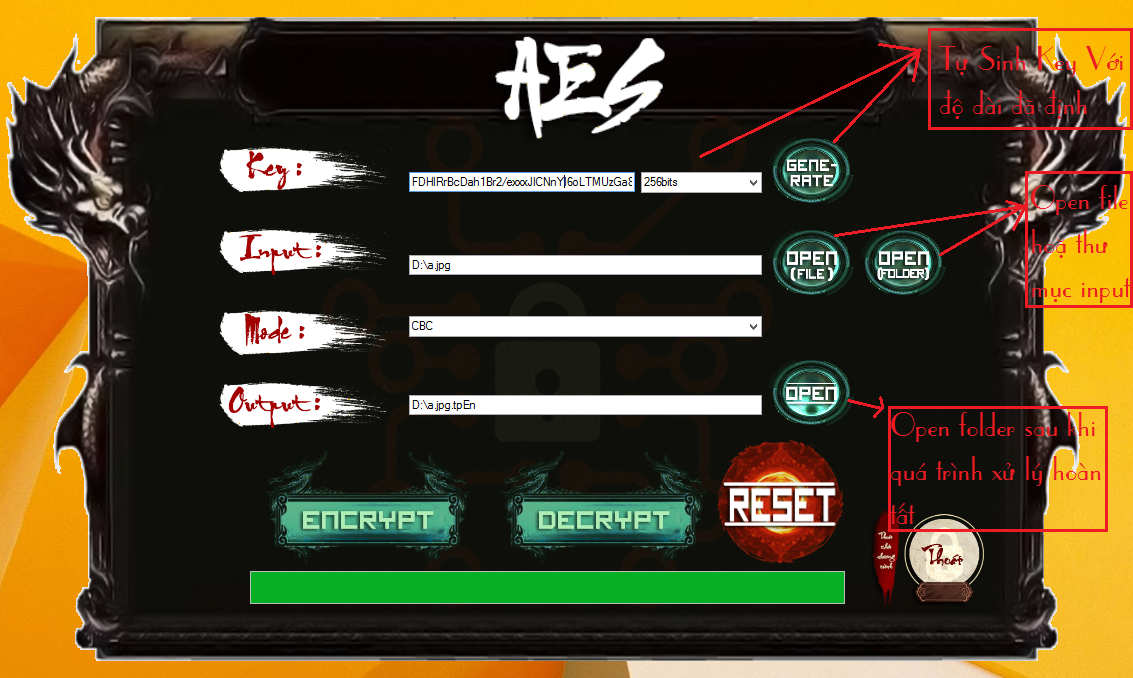
\includegraphics[scale=0.4]{AES_MOTATINHNANG}
 		
 		Phần Input File : có thể mã hóa hầu hết tất cả các file như: hình ảnh, âm thanh, video, pdf, các file dạng văn bản… Còn có thể mã hóa tập tin nén dạng zip,thư mục,rar…\\
 		
 		
		Phần Input Key : có thể nhập key bất kỳ hoặc chọn Generate key(từ độ dài định trước) để random một key bất kì.\\
		
		
		Phần Output File: mặc định chọn nơi lưu file ciphertext là nơi chọn file plaintext để mã hóa, file ciphertext có đuôi .tpEn\\
			
			
		Nhấn Encrypt để bắt đầu mã hóa.
 		\subsubsection{Phần giải mã}\\
 		Phần Input File: chọn file có đuôi.tpEn để giải mã.\\
 		
		Phần Input Key: nhập key ở phần mã hóa.\\
			
		Phần Output File: xuất ra file plaintext ban đầu.\\
		
		Ấn Decrypt để tiến hành giải mã.
%%%%%%%%%%%%%%%%%%%%%%%%%%%%%%%%%%%%%%%%%%%%%%%%%%%%%%%%%%%%%%%%%%%%%%%%%%%%%%5
\section{Phân tích và kết luận}
	
	\subsection{Phân tích}
	\begin{itemize}
		\item Giải thuật DES : đã hóa thành công tất cả các file dựa trên việc chia các file thành block nhỏ.
		\item Giải thuật RSA : mã hóa thành công các file có kích thước nhỏ, và xử lý khóa có chiều dài ngắn.
		\item Hàm băm MD-5 : mã hóa thành công hầu hết các file và các đoạn text.
		\item Giải thuật AES : đã hóa thành công tất cả các file.
	\end{itemize}
	
	\subsection{Kết luận}
	\begin{itemize}
		\item Kết quả dạt được:\\
		Đã mã hóa và giải mã thành công các file có kích thước vừa và nhỏ.

		\item Hạn chế: \\
		Thời gian mã hóa và giải mã các file có kích thước lớn khá lâu.\\
		
		Ở giải thuật RSA, khi chọn key có kích thước lớn (ví dụ:4096) thì tốc độ mã hóa chậm. \\
	
	\end{itemize}	
	
	
\section{Hướng phát triển}
	Cải thiện thời gian mã hóa cũng như giải mã các tập tin có kích thước lớn của các giải thuật nêu trên.\\
	
Ở giải thuật RSA, tìm kiếm biện pháp giải quyết vấn đề khi sử dụng key có kích thước lớn để mã hóa tập tin.(ví dụ dùng multi-threading)\\

Cải thiện giao diện chương trình…

\section{Tài liệu tham khảo}

https://vi.wikipedia.org/wiki/AES\_(m\%C3\%A3\_h\%C3\%B3a)\\
https://vi.wikipedia.org/wiki/MD5\\
https://vi.wikipedia.org/wiki/RSA\_(m\%C3\%A3\_h\%C3\%B3a)\\
https://en.wikipedia.org/wiki/Data_Encryption_Standard\\


	
\end{document}